\chapter{Register File}

There are only two remaining parts of the decode stage: the register file (this week) and the buffer (next week).
\begin{wrapfigure}{L}{1in}
\caption{Register file.}\label{fig:regfile}
\begin{center}
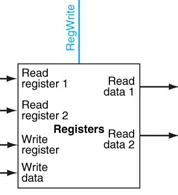
\includegraphics[width=1in]{../images/regfile.png}
\end{center}
\end{wrapfigure}

Consider the interface of the register file, as depicted in Figure~\ref{fig:regfile}.  Note that inputs enter on the left, controls on the top, and outputs exit on the right.  We will be making a unit with 32 registers of size WORD.  Also note that clock and reset are not included, but should be implicit, since we are building memory.  We will need to read two registers at a time to do our arithmetic on two inputs (called A and B\footnote{These are the old names that was pretty universally used.  I keep using them because it is a tip of the hat to where we came from.})  We will have one value to input, but only if write is asserted.  Be careful of the timing - since the update is on the negative edge, just like the buffer which will drive it, a delay will speed things up.

Notice that the input (writing to the registers) and the output (reading from the registers) will not be done at the same time due to the clock edge they happen on.  This ensures that the data can update and be read in the same clock cycle.  This will also require that the updating stage, called write back (WB or w/b for short), be a very small stage.  Write back indeed is small, being composed of just one mux and the inputs to the registers.

One final note, it would be tempting to take the write signal for the register file directly from control, but don't!  The write signal, the write address, and the write value must all arrive at the same time or you will update the wrong value or to the wrong place. We thus will pass all three signals along down the pipeline so the buffers at each stage will keep them coordinated.  This is really important.  The last buffer, mem-wb, will then be used to drive the update of the register file during the write back stage, when we know the values are good.

\section{Your Assignment}

You are to:
\begin{enumerate}
\item Finish the register file.
\item Write a testbench for the register file, run a simulation and generate a timing diagram.
\item  Write up a lab report in \LaTeX\ following the lab format in \verb1LabN.tex1 and generate a pdf file.
\item Upload the pdf and all the Verilog files to the course LMS.
\end{enumerate} 